\chapter{胸部DCE-MRI压缩感知模型中时间稀疏项的量化评估}
\label{chap:qetsr}
磁共振动态对比增强涉及注入顺磁对比剂期间和之后连续采集$T_1$加权MR图像\cite{Yankeelov2009}。对比剂通过改变组织固有的驰豫率来增加不同组织之间的对比度。在序列图像中,每个图像体素都会产生一个强度时间曲线,可以用于估计生理参数,例如体积转移常数\kt 和血管外细胞体积分数\Ve 等。高时间分辨率和高空间分辨率都有利于DCE-MRI, 高时间分辨率有利于精确地定量分析,而高空间分辨率有助于医生的临床阅读。但是,对重复高信噪比图像的要求限制了传统数据采集方法同时提高时间和空间分辨率。

为了加速动态MR成像,一种常用的方法来平衡空间和时间分辨率之间的权衡是在每一帧图像上进行下采样。许多成功的算法都用到了这个想法,如keyhole\cite{van1993}, k-t FOCUSS\cite{focuss}, k-t BLAST和k-t SENSE\cite{Jeffrey2003k}。但是,这些方法所重建的图像通常信噪比低,而且在高下采样率时有严重的伪影。

压缩感知是一种加速MR成像的新方法\cite{Donoho2006Compressed,Candes2006Robust}。压缩感知可以用比传统加速方法少的Fourier数据精确地重建出MR图像,从而减轻数据获取的负担,加速成像。根据压缩感知的理论,MR图像的重建可以建模为一个约束优化问题。这个优化模型一般分为两项,一项是数据项,另一项是稀疏项。数据项保证了重建后的图像与采集到的下采样数据的一致性,而稀疏项则假设图像在某个变换域下存在稀疏表示。对于动态图像而言,由于图像中的大部分在时间上是保持不变的,因此最显著的冗余性(即稀疏性)经常体现在时间方向上。

压缩感知在癌症MR成像中有着很大的应用潜力\cite{smith2013},因为很多癌症MR成像的协议都是动态的。目前,压缩感知在动态MRI中已经有很多成功的应用,如k-t SPARSE\cite{lustig2006}、k-t SLR\cite{Sajan2011Accelerated}、iGRASP\cite{igrasp}等。比如,Han等展示了基于压缩感知加速的Cartesian采样FLASH (fast low angle shot) \cite{han}序列在动物模型的DCE-MRI时空分辨率的增强。Chen\cite{chen}等比较了压缩感知重建中4种不同的时间方向TV正则项的效果,并且将其应用在胸部DCE-MRI中。Ji和Lang\cite{ji2008}使用时间方向的差分算子来增强空间信号的分辨率。Smith\cite{smith2011,smith2012}等展示了空间方向的TV稀疏项在大量随机生成的采样方案中量化参数的预期方差。虽然压缩感知已经应用于胸部DCE-MRI中,但是目前还没有研究通过量化分析的方式来比较不同时间方向的稀疏项在DCE-MRI中的表现。因此,对于定量胸部DCE-MRI,不同时间方向的稀疏项对重建误差的影响是未知的。

在压缩感知应用于临床肿瘤成像之前,其可靠性和准确性的研究是必要的。本章的主要目的是通过量化分析的方式来比较和评估5中不同的时间方向的稀疏项,它们分别是:
\begin{enumerate}
	\item Fourier变换的$l_1$范数 (Fourier transform, FT);
	\item Haar小波变换的$l_1$范数 (Haar wavelet transform, WT);
	\item TV;
	\item 二阶TGV ($\textrm{TGV}_{\alpha}^2$);
	\item 核范数 (NN)。
\end{enumerate}
我们假设这些稀疏项的在基于压缩感知重建中的表现是不同的,即重建图像的信噪比和组织参数的准确性会有差异。

\section{图像重建模型}
我们将重建的动态MR图像记为$X\in \mathbb{C}^{N_1\times N_2\times d}$,其中空间方向的维度为$N_1\times N_2$,而时间方向的维度为$d$。则带噪声的动态MR采样相当于:
$$B=AX+\epsilon,$$
其中$A=\mathcal{M}\cdot \mathcal{F}$是采样矩阵,$\mathcal{F}$是对于每一帧图像的二维Fourier变换,$\mathcal{M}$是每一帧图像的下采样矩阵,$\epsilon$为高斯白噪声。于是动态MR的压缩感知即是从下采样数据$B$中恢复出$X$,其重建模型为:
\begin{equation}
\hat{X} = \argmin_X \frac{1}{2}\|AX-B\|_\mathrm{F}^2 + \alpha\|\mathcal{S}_tX\|,
\end{equation}
其中$\alpha>0$是平衡数据项和稀疏项的参数,$F$是Forbenius范数,而$\mathcal{S}_t$是某个时间方向的稀疏项。极小化稀疏项可以保证重建图像的稀疏性,而极小化数据项可以保证数据的一致性。

\subsection{基于Fourier变换的重建模型}
动态MRI经常在时间方向上表现出冗余性,有时这种冗余表现为周期性,因此时间方向上的一维Fourier变换可以对信号进行稀疏表示。信号越是表现出周期性,其在Fourier变换域中就越稀疏。并且由于下采样的去噪效应,一个非周期性的带噪信号在Fourier域也是可压缩的。比如,在心脏电影成像中,由于心脏搏动的周期性,图像可以很好地用时间方向的Fourier变换进行稀疏表示。在k-t SPARSE\cite{Lustig2010Sparse}中,作者使用了空间上的小波变换和时间上的Fourier变换作为压缩感知重建的稀疏项。记$\mathcal{F}_t$为一维时间上的Fourier变换,我们可以得到模型:
\begin{equation}
\hat{X} = \argmin_X \frac{1}{2}\|AX-B\|_\mathrm{F}^2 + \alpha ||\mathcal{F}_t X||_1.
\end{equation}

\subsection{基于Haar小波变换的重建模型}
小波变换是基于压缩感知重建中常用的稀疏表示。对于MR图像而言,Haar小波有两个感兴趣特征。第一,分片常数的信号在Haar小波的表示下是稀疏的。第二,Haar小波变换和MR图像的采集域,即Fourier域有着高非相干性。根据压缩感知理论,这意味着对于给定的下采样率,Haar小波变换可以获得更好的重建图像。比如,k-t SPARSE\cite{Lustig2010Sparse}将空间小波变换成功地应用在了心脏电影成像中。记$\mathcal{W}_t$为一维时间方向的Haar小波变换,我们可以得到模型:
\begin{equation}
\hat{X} = \argmin_X \frac{1}{2}\|AX-B\|_\mathrm{F}^2 + \alpha ||\mathcal{W}_t X||_1.
\end{equation}

\subsection{基于TV的重建模型}
在压缩感知应用在MR成像的第一篇文章中,Lustig\cite{Lustig2008Compressed}在模型中使用了有限差分作为图像的稀疏表示。离散TV算子将时间和空间上的差分算子进行加权组合,本质上是将图像用梯度进行稀疏表示。TV泛函最初被应用于图像去噪中\cite{rof},最近也经常应用于压缩感知重建中。离散TV算子和Fourier域有着最大的非相干性,因此,对于给定的下采样率,会比其他稀疏表示得到更好的重建图像。但实际上,使用TV正则项经常会导致重建后的图像出现阶梯效应。这是因为真实的MR图像中并不是完美的分片常数,而是存在高阶信息。当这些高阶信息用分片常数函数来刻画时,在重建的过程中,为了使得图像在梯度域中稀疏,最小的梯度系数会被减小到零,因此会损失很多高阶信息,从而出现阶梯效应。在k-t SLR\cite{Sajan2011Accelerated}中,作者使用了三维TV变换:
$$\|\cdot\|_\mathrm{3DTV} = \|\nabla_3\cdot\|_1,$$
而
$$|\nabla_3\cdot|=\sqrt{(\nabla_x \cdot)^2 + (\nabla_y \cdot)^2 + (\nabla_t \cdot)^2},$$
其中$\nabla_x,\nabla_y$和$\nabla_t$分别为$x,y$和$t$方向上的梯度算子。也有文献只使用了时间方向上的梯度算子就取得了很好的效果,如DLTG\cite{caballero2014dictionary}和iGRASP\cite{igrasp}。在本文中,我们仅考虑时间方向的梯度算子并评估以下模型的表现:
\begin{equation}
\hat{X} = \argmin_X \frac{1}{2}\|AX-B\|_\mathrm{F}^2 + \alpha\|\nabla_t X\|_1.
\end{equation}

\subsection{基于二阶TGV的重建模型}
如上所言,有限差分算子可以很好地对MR图像进行稀疏表示,但是也会带来阶梯效应。因此,Bredies\cite{bredies2010total}等提出了基于高阶导数信息的TGV泛函,可以更好地对图像中的高阶信息进行建模,消除阶梯效应。对于二维图像$u\in \mathbb{C}^{N_1\times N_2}$,其离散二阶TGV的定义如下:
$$\mathrm{TGV}_\alpha^2(u)=\min_{\omega\in \mathrm{BD}(\Omega)}\alpha_1\|\nabla_3 u-\omega\|_1 + \alpha_0\|\mathcal{E}(\omega)\|_1,$$
其中$\nabla\cdot=(\nabla_x\cdot, \nabla_y\cdot)$一阶有限差分算子,$\mathcal{E}(\omega)=\frac{1}{2}(\nabla_3\omega+\nabla_3\omega^{T})$是对称梯度算子,$\mathrm{BD}(\Omega)$ 是有界形变函数空间。

从定义中可以看出,$\mathrm{TGV}_\alpha^2$是TV的高阶推广,可以很好地保持图像一阶和二阶导数之间的平衡。因此$\mathrm{TGV}_\alpha^2$比TV更适合建模图像中的光滑部分。在压缩感知模型中,使用$\mathrm{TGV}_\alpha^2$可以在保持边缘的同时减少阶梯效应。在本文中,我们只考虑时间方向的$\mathrm{TGV}_\alpha^2$:
\begin{equation}
\hat{X} = \argmin_X \frac{1}{2}\|AX-B\|_\mathrm{F}^2+\mathrm{TGV}_\alpha^2(X),
\end{equation}
这里$\nabla \omega = \nabla_t \omega$,$\omega\in \mathbb{C}^{N_1N_2d}$.

\subsection{基于核范数的重建模型}
低秩矩阵补全的想法也被应用在动态MR重建中。这时我们将动态MR图像视为一个时空矩阵,每一帧图像则为时空矩阵中的一列,每一个像素点为时空矩阵的一行。由于动态图像时间和空间上的相关性,这样的矩阵可以用低秩模型来刻画。因此,将压缩感知和低秩矩阵补全结合在一起可以进一步加快成像速度。在k-t SLR中,作者在模型中使用核范数,并在体膜数据和心脏灌注数据中取得了显著的提高。核范数记为$\|X\|_*$,是矩阵$X$所有奇异值的和。本文我们考虑如下模型:
\begin{equation}
\hat{X} = \argmin_X{\frac{1}{2}\|AX-B\|^2_\mathrm{F} + \alpha\|X\|_*}.
\end{equation}

\section{图像重建快速算法}
\subsection{FISTA快速算法}
在本文中,所有模型都使用FISTA\cite{fista}算法进行求解。FISTA是一种算子分裂算法,是压缩感知重建中常用的快速算法,可以有效地求解如下形式的模型:
\begin{equation}
\hat{x} = \argmin_{x \in \mathbb{\mathbb{C}}^n} f(x) + g(x),
\end{equation}
其中,$f$是光滑的凸函数,其Lipschitz常数为$L_f$;$g$是凸函数,可能是非光滑的。FISTA的迭代过程算法\ref{alg:qetsr}所示。这里$\prox_\tau(g)(u)$是函数$g(x)$在点$x$的临近算子,定义为:
\begin{equation}
\prox_\tau(g)(u)=\argmin_x{g(u)+\frac{1}{2\tau}}\|u-x\|_2^2.
\label{equ:prox}
\end{equation}
而投影算子$\mathscr{P}$定义为:
\begin{equation}
x=\mathscr{P}(x,[l_1,l_2]) =
\left\{
\begin{array}{ll}
x, \quad \mbox{if} \quad l_1\leq x\leq l_2; \\
l, \quad \mbox{if} \quad x<l_1;\\
u, \quad \mbox{if} \quad x>l_2.\\
\end{array}\right.
\end{equation}

\begin{algorithm}
	\caption{稀疏重建的FISTA算法}
	\label{alg:qetsr}
	\begin{algorithmic}
		\REQUIRE $\tau, l_1, l_2, t^1=1, x^0=r^1$;
		\INDSTATE[-1.25] \textbf{迭代:根据以下步骤更新参数:}	
		\STATE 1. $\bar{x}=r^n-\tau A^*(Ax-b)$;
		\STATE 2. $x^n=\prox_{\tau}(g)(\bar{x})$;
		\STATE 3. $x^n=\mathscr{P}(x^n,[l_1,l_2])$
		\STATE 4. $t^{n+1}=(1+\sqrt{1+4(t^n)^2})/2$;
		\STATE 5. $r^{n+1}=x^n+\frac{t^n-1}{t^{n+1}}(x^n-x^{n-1})$;
		\ENSURE $x^{n+1}$。
	\end{algorithmic}
\end{algorithm}

FISTA中最重要的一步是找到高效的算法求解临近点子问题。由于在压缩感知模型中,我们通常使用$l_1$范数作为稀疏项,临近点问题可以由软阈值收缩求解。比如,令$g(u) = \|u\|_1$,则方程(\ref{equ:prox})变为:
\begin{equation}
\prox_\tau(g)(u)=\argmin_u{\|u\|_1+\frac{1}{2\tau}}\|u-x\|_2^2.
\label{equ:proxl1}
\end{equation}
方程(\ref{equ:proxl1})的解为
\begin{equation}
u=\mathscr{S}_{\tau}(x),
\end{equation}
其中软阈值收缩算子$\mathscr{S}_{\tau}:\mathbb{R}^n\xrightarrow{} \mathbb{R}^n$的定义为:
\begin{equation}
\mathscr{S}_{\tau}(x)=
\mathrm{max}(0, x-\tau).
\end{equation}
当$g(u)$为TV或者$\mathrm{TGV}_\alpha^2$时,临近点问题不能用简单地软阈值收缩进行求解,因此我们用Primal-Dual算法进行求解。Primal-Dual算法的详细流程请参考第\ref{chap:tgvlr}章。

\subsection{模型参数的选择}
压缩感知模型中,参数的选择是至关重要的,因为只有在每个模型都达到最优解时的比较才是有意义的。在本文的数值实验中,所有胸部DCE-MRI数据都被缩放到[0,1],这样有助于简化调参。表\ref{tab:params4}显示了以上所有模型所用的参数。其中$\alpha$是稀疏项的权重,iter是算法的迭代次数,$\sigma$,$\tau$和$\lambda$分别是TV或$\mathrm{TGV}_\alpha^2$模型中,一阶迭代步长、二阶迭代步长和数据项的权重。参数的调节方法如下:我们从很低的权重开始 ($\alpha=10^{-5}$)并且逐步增加权重的大小直到空间伪影在视觉上从重建的图像中消失。在每一步迭代中,我们跟踪连续两次输出图像的相对差值,直到其小于预设的阈值 ($10^{-3}$)。

\begin{table}
\setlength{\belowcaptionskip}{10pt}
\caption{各个模型所使用的参数}
\centering
\begin{tabular}{|l|l|l|l|l|l|}
\hline
\hline
稀疏项 & $\alpha$ & iter & $\sigma$ & $\tau$ & $\lambda$\\
\hline
FT & 0.059 & 35 & - & - & -\\
\hline
WT & 0.008 & 60 & - & - & -\\
\hline
TV & 0.5 & 100 & 0.2 & 0.2 & 0.5\\
\hline
TGV$_{\alpha}^2$ & 0.5 & 100 & 0.2 & 0.2 & 0.5\\
\hline
NN & 0.3 & 40 & - & - & -\\
\hline
\end{tabular}
\label{tab:params4}
\end{table}

\section{数值实验数据与评价方法}
\subsection{数值实验数据}
我们回顾性地将所有模型应用于活体胸部DCE-MRI数据上,这些数据经过了机构审查委员会的批准。数据使用Philips公司的Achieve 3T扫描仪通过破坏性梯度回波序列(Spoiled Gradient Recalled Echo, SPGRE)获取,重复时间$T_\mathrm{R}$为4.33 ms,回波时间$T_\mathrm{E}$为2.12 ms,偏转角为12$^\circ$。数据的维度为$192\times 192\times 10\times 105$,其中相位编码和频率编码均为192,切片数量为10,动态数量为105。空间分辨率为1.33 mm $\times$ 1.33 mm $\times$ 5 mm,视野大小为256 mm $\times$ 256 mm $\times$ 50 mm。更详细的成像细节请参考文献\cite{xia}。

数据通过Cartesian全采样模式获得,然后通过一些列的随机采样模式进行回顾性下采样。虽然前瞻性下采样更加符合现实,但是前瞻性地获取上百种不同的下采样模式是不切实际的。为了缩小文章的重点,我们只选取了肿瘤中心所在的切片。在我们的数据中,这是第6个切片。同时在所有的重建中,我们切除了胸腔的后边部分来增加图像的稀疏性,这是因为跳动的心脏会在相位编码方向上产生伪影,从而降低重建图像的信噪比。切掉胸腔的过程可以在下采样数据中进行,因为即使在充满伪影的图像中,胸腔也是很容易被划分出来的。最终图像的维度为$192\times 128\times 105$。

我们生成了200个不同的Cartesian下采样模式,每个采样模式的维度都和数据相同,即$192\times 128\times 105$。在每一帧图像上,我们对低频区域进行全采样,对高频区域进行随机采样。具体来说,我们在k-space中选取中心窗口大小为20的区域作为低频区域,而在外围的高频区域,我们随机选择一些相位编码线,使得总体来说外围的每一条相位编码被选取的次数相同。这200个下采样模式的平均下采样率为4.5。这里我们选择4.5是因为Cartesian采样的固有限制,更高的采样率可以使用non-Cartesian采样模式获得,但这不在本文考虑范围内。图\ref{fig:mask1}显示了一个Cartesian采样模式的例子。

\begin{figure}[htbp]
\centering
  \setlength{\abovecaptionskip}{20pt}
  \setlength{\belowcaptionskip}{20pt}  
  \begin{overpic}[scale=0.6]{img/qetsr/figure1.eps}
    \put(-7,34){\large \color{black}{\bf $k_y$}}
    \put(45,34){\large \color{black}{\bf $k_y$}}
    \put(18,-5){\large \color{black}{\bf $k_t$}}
    \put(74,-5){\large \color{black}{\bf $k_x$}}
  \end{overpic}
  \\
\caption{Cartesian采样模式的例子。左图显示的是所有帧的采样模式,右图显示的是某一帧的采样模式。右图的二维采样模式通过左图的一列在$x$方向上重复得到。在每一帧图像上,中心的低维区域进行全采样,而外围的高维区域进行随机采样。整体的下采样在4.5左右。}
\label{fig:mask1}
\end{figure}

\subsection{采样模式与评价方法}
我们使用两种方法对重建结果进行评估。首先,为了和之前的文献一致,我们使用基于图像像素值本身的信噪比(SER)对图像进行评估。SER的定义如下:
\begin{equation}
\mathrm{SER} = -10 \log_{10}\frac{\|X_\mathrm{rec}-X_\mathrm{ori}\|_\mathrm{F}^2}{\|X_\mathrm{ori}\|_\mathrm{F}^2},
\end{equation}
其中$X_{\mathrm{ori}}$为全采样图像,即原图像,$X_{\mathrm{rec}}$为算法重建后的图像。

我们使用的第二种评估方法是通过DCE-MRI的药代动力学(pharmacokinetic)模型来进行定量分析。本文我们使用最常用的标准Tofts-Kely模型\cite{tofts}来计算\kt 和\Ve 的值。首先我们分别计算全采样和重建图像\kt 和\Ve,然后用一致性相关系数(concordance correlation coefficients,CCC)来度量他们之间的相似性程度。这是DCE-MRI中进行定量参数分析的常用方法。在统计学上,CCC的定义如下:
\begin{equation}
\mathrm{CCC} = \frac{2\sigma_\mathrm{ori} \sigma_\mathrm{rec}}{\sigma_\mathrm{ori}^2+\sigma_\mathrm{rec}^2+(\mu_\mathrm{ori}-\mu_\mathrm{rec})^2},
\end{equation}
其中$\mu_\mathrm{ori}$和$\mu_\mathrm{rec}$分别为全采样图像和压缩感知重建图像\kt 或者\Ve 的期望,$\sigma_\mathrm{ori}$和$\sigma_\mathrm{rec}$是相对应的方差.

为了从视觉上直观地评估重建图像时间剖面的准确性,我们计算了重建图像肿瘤区域的时间曲线相对于全采样图像之间的差异。我们首先手动将肿瘤区域分割出来,形成一个掩膜,并应用于所有重建图像。我们也分别计算了全采样图像和重建图像肿瘤区域内\kt 和\Ve 的平均值,并用Bland-Altman图来显示其一致性。

重建程序全部使用MATLAB语言编写,DCE-MRI的参数分析使用Julia语言的\texttt{DCEMRI.jl}\cite{Smith2015}工具包运行。所有数值实验均在双核Xeon E5-2665 2.40 GHz,20 GB内存的工作站上运行,MATLAB版本为2015b (Mathworks, Natick, MA),Julia版本为0.4.3。
%程序已经开源,详细程序请参考网址\url{https://github.com/chixindebaoyu/qetsr}。

\section{数值实验结果}
\subsection{重建图像质量}
我们首先评估了这5种时间方向的稀疏项在图像质量上的表现。表\ref{tab:result}的第2列显示了200个不同Cartesian采样模式下重建图像的平均SER。可以看出,在5种稀疏项中,核范数得到了最高的SER(29.1),小波变换的SER最低(21.8),而Fourier变换的效果介于小波变换和TV(27.7)之间。其中,TGV$_\alpha^2$(27.8)与TV有着相似的表现。

\begin{table}
\caption{200个Cartesian采样模式重建的均值SER与CCC}
\centering
\begin{tabular}{|l|l|l|l|}
\hline
\hline
\multirow{2}*{稀疏项}&\multirow{2}*{SER}&\multicolumn{2}{c|}{CCC} \\
\cline{3-4}
~ & ~ & \kt & \Ve \\
\hline
Zerofilled & 15.1 & 0.694 & 0.636\\
\hline
FT & 26.4 & 0.763 & 0.575\\
\hline
WT & 21.8 & 0.878 & 0.733\\
\hline
TV & 27.7 & \textbf{0.974} & 0.916\\
\hline
TGV$_\alpha^2$ & 27.8 & \textbf{0.974} & \textbf{0.917}\\
\hline
NN & \textbf{29.1} & 0.842 & 0.799\\

\hline
\end{tabular}
\label{tab:result}
\end{table}

图\ref{fig:recon}(a)显示了第1个Cartesian采样模式下5种时间稀疏项重建结果的第105帧图像。图中红色箭头显示,背景伪影在TGV$_\alpha^2$和TV中依然存在,而NN基本消除了伪影。虽然FT和WT也很好地抑制了伪影,但是它们在肿瘤部分重建的表现是最差的。

图\ref{fig:recon}(b)显示了同样Cartesian采样模式下重建结果的第1帧图像。图中红色箭头显示,在视觉上TGV$_\alpha^2$和TV重建肿瘤的效果是最好的,这也是我们之后进行定量参数分析所用到的部分。FT和WT在重建肿瘤方面的表现是最差的,而NN虽然SER最高,但从视觉上看,肿瘤部分的误差却高于TGV$_\alpha^2$和TV。

\begin{figure}[htbp]
\centerline{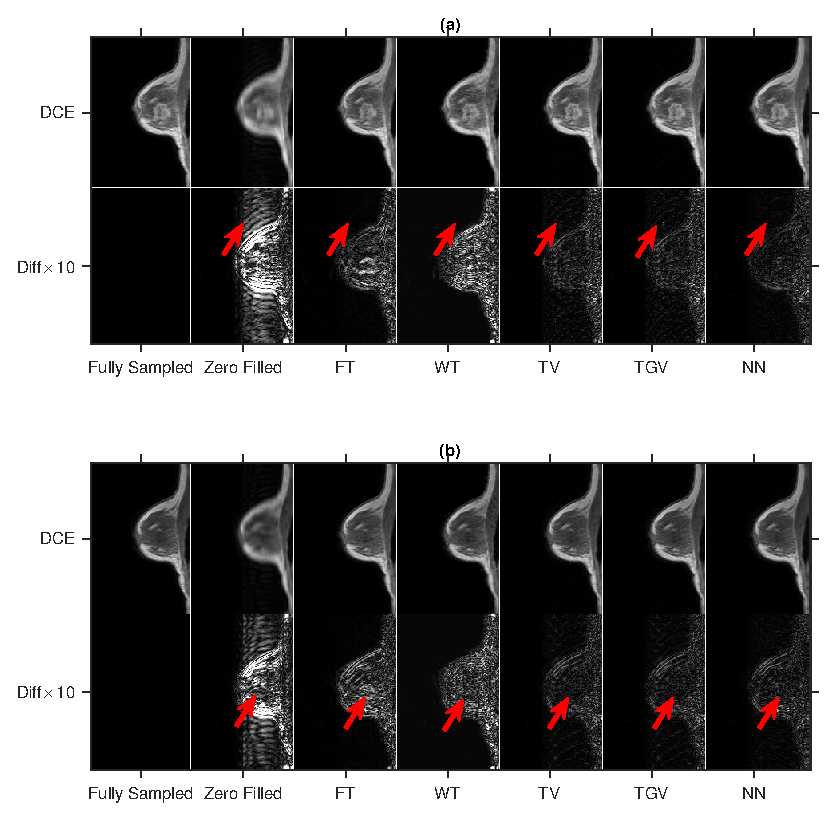
\includegraphics[width=1\textwidth]{img/qetsr/figure2.eps}}
\caption{
第一个Cartesian采样模式的重建结果。(a)第105帧;(b)第1帧。在每一个子图中,第一行显示的分别是全采样、Zerofilled、WT、FT、TV、TGV$_{\alpha}^2$和NN的重建图像,第二行是相应的与全采样图像之间的差值图像。为了使得差值图像有更好的视觉效果,我们将每一张差值图像的像素值都放大了10倍。图中的红色的箭头显示,在视觉上TV和TGV$_\alpha^2$模型重建肿瘤的效果是最好的,而在NN去除背景伪影方面表现最好。
}
\label{fig:recon}
\end{figure}

图\ref{fig:boxplot}显示了重建图像SER的箱型图。我们可以观察到,对于每个稀疏项而言,SER的方差都相对很小。因此除了TV和TGV$_\alpha^2$之间,所有结果在统计学上都有显著差异。从箱型图中也可以看出,NN的平均SER最高(29.1),而WT的SER最低(21.8)。

\begin{figure}[htbp]
\centerline{
    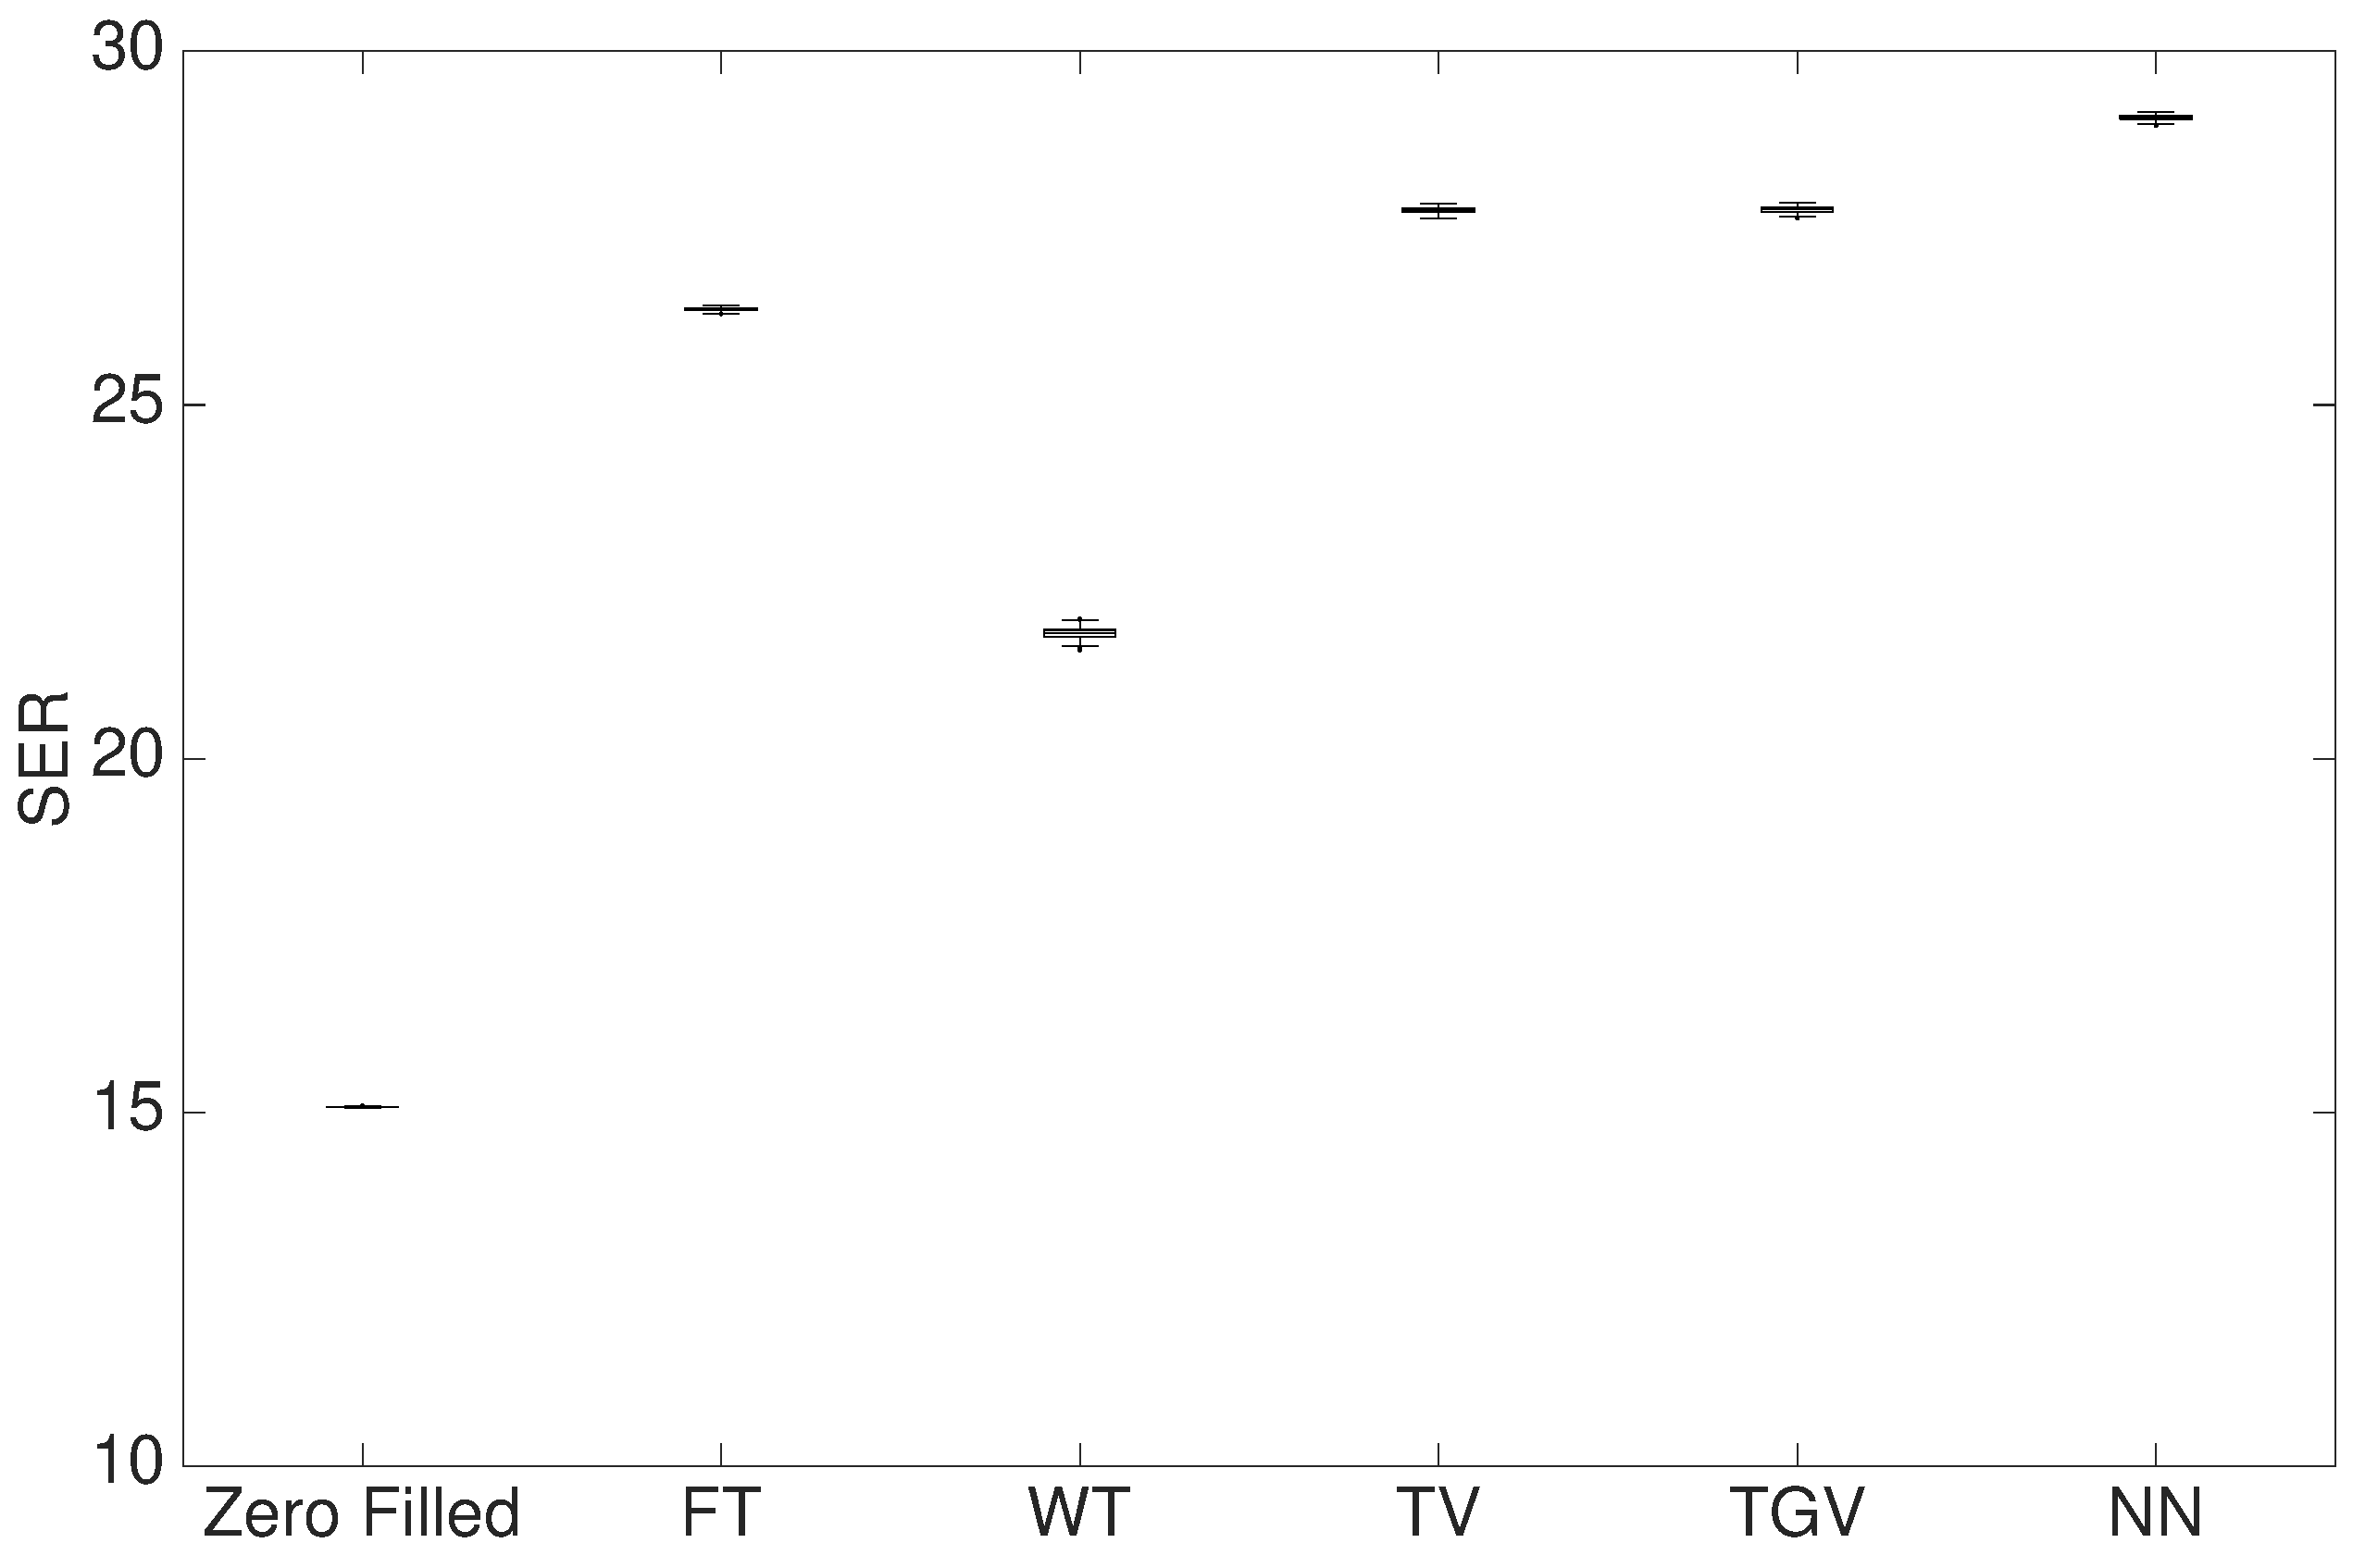
\includegraphics[width=1\textwidth]{img/qetsr/figure3.eps}
}
\caption{
重建图像SER的箱型图。除了TV和TGV$_\alpha^2$之间,所有结果在统计学上都有显著差异。从箱型图中可以看出,NN的平均SER最高(29.1),而WT的SER最低(21.8)。
}
\label{fig:boxplot}
\end{figure}

\subsection{定量参数精度}
表\ref{tab:result}的第3列和第4列分别显示了5中稀疏项重建结果的\kt 和\Ve 的CCC。TV和TGV$_\alpha^2$都得到了最高的参数精度,其中TV的参数精度分别为0.974和0.916,而TGV$_\alpha^2$的精度分别为0.974和0.917。虽然NN得到了最高的SER(29.1),但其参数精度却不是最高的,分别为0.842和0.799。同样的现象也发生在WT与FT上,WT的SER(21.8)比FT(26.4)低,但是其参数精度则比FT高。

图\ref{fig:zoom}显示了\kt 和\Ve 参数图肿瘤部分放大后的图像。在视觉上,TV和TGV$_\alpha^2$都精确地重建出\kt 和\Ve,与全采样的参数图最接近,没有任何去噪与模糊的效果。而NN的参数图像则变得模糊,有过平滑的效果。

\begin{figure}[htbp]
\centerline{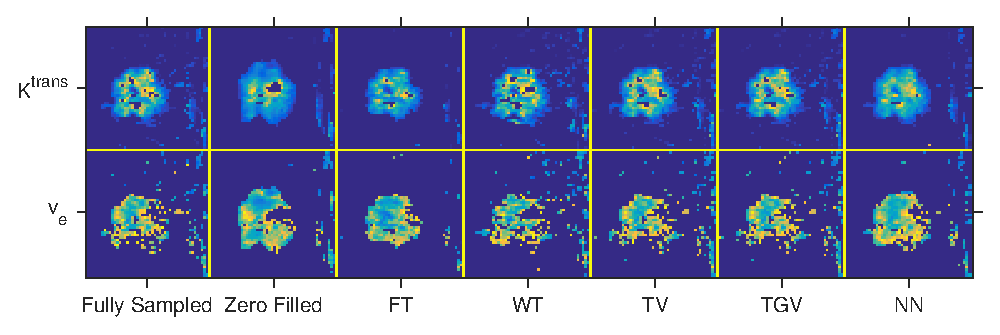
\includegraphics[width=1.0\textwidth]{img/qetsr/figure4.eps}}
\centering
\caption{
\kt 和\Ve 参数肿瘤部分放大后的图像。第一行从左到右依次显示了全采样、Zerofilled、WT、FT、TV和TGV$_{\alpha}^2$的\kt 图像;第二行是相应的\Ve 图像。在视觉上,TV和TGV$_{\alpha}^2$与全采样的参数图像最接近。
}
\label{fig:zoom}
\end{figure}

图\ref{fig:baplot}显示了5种稀疏项\kt 和\Ve 的Bland-Altman图。从图中可以看出,TV和TGV$_{\alpha}^2$得到了几乎无偏差的\kt 和\Ve,而WT、FT和NN都低估了\kt 和\Ve 的值。虽然从表\ref{tab:result}中可以看出,WT得到了相对准确地CCC,但图\ref{fig:baplot}表明,WT也严重低估了肿瘤部分的均值。

\begin{figure}[htbp]
\centerline{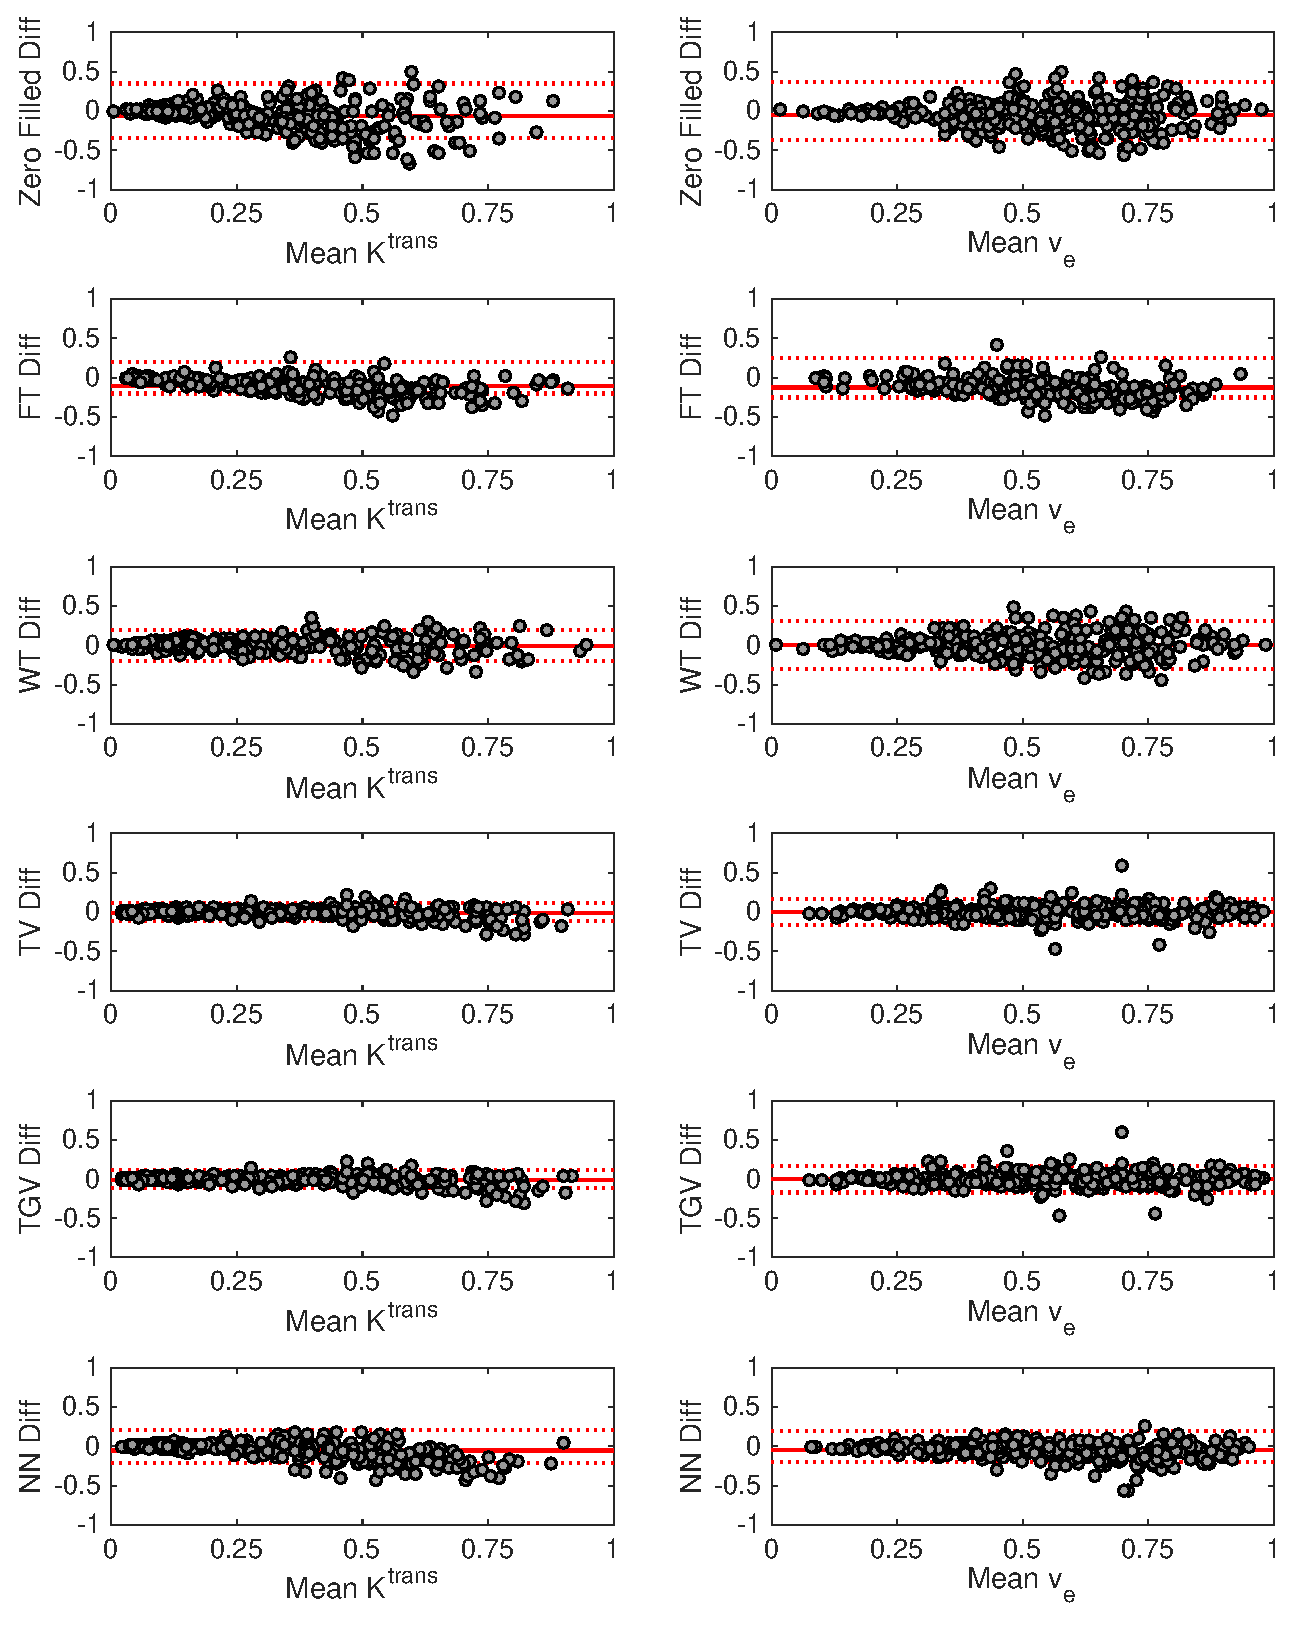
\includegraphics[width=0.9\textwidth]{img/qetsr/figure5.eps}}
\centering
\caption{
5种稀疏项\kt 和\Ve 的Bland-Altman图。第一列为\kt,第二列为\Ve。从上到下依次为WT、FT、TV、TGV$_{\alpha}^2$和NN。TV和TGV$_{\alpha}^2$得到了最准确并且偏差最小的参数。FT的偏差值最大,WT的参数最不准确。NN虽然低估了参数值,但其偏差值较小。
}
\label{fig:baplot}
\end{figure}

图\ref{fig:curves}显示了全采样图像与重建图像肿瘤区域像素时间曲线的比较。图\ref{fig:curves}(a)是肿瘤区域所有像素平均值的时间曲线,而图\ref{fig:curves}(b)是肿瘤中心像素点(96,96)的时间曲线。从图\ref{fig:curves}中可以看出,Zerofilled图像最初5帧的重建结果是准确的,但是当注入CA之后,像素值就被低估了,导致SER、\kt 和\Ve 的减小。WT低估了所有帧的肿瘤区域的平均像素值。在图\ref{fig:curves}(a)中,FT的最初5帧和最后5帧的拟合效果很差,而且整体体现出了振荡的效应。这一点从图\ref{fig:curves}(b)中可以更明显地观察到。TGV$_{\alpha}^2$和TV最好地拟合了肿瘤区域平均像素值和单个像素值的时间曲线。在最初的几帧中,NN高估了平均像素值,这也影响了其最终\kt 和\Ve 的准确性。

\begin{figure}[htbp]
\centerline
{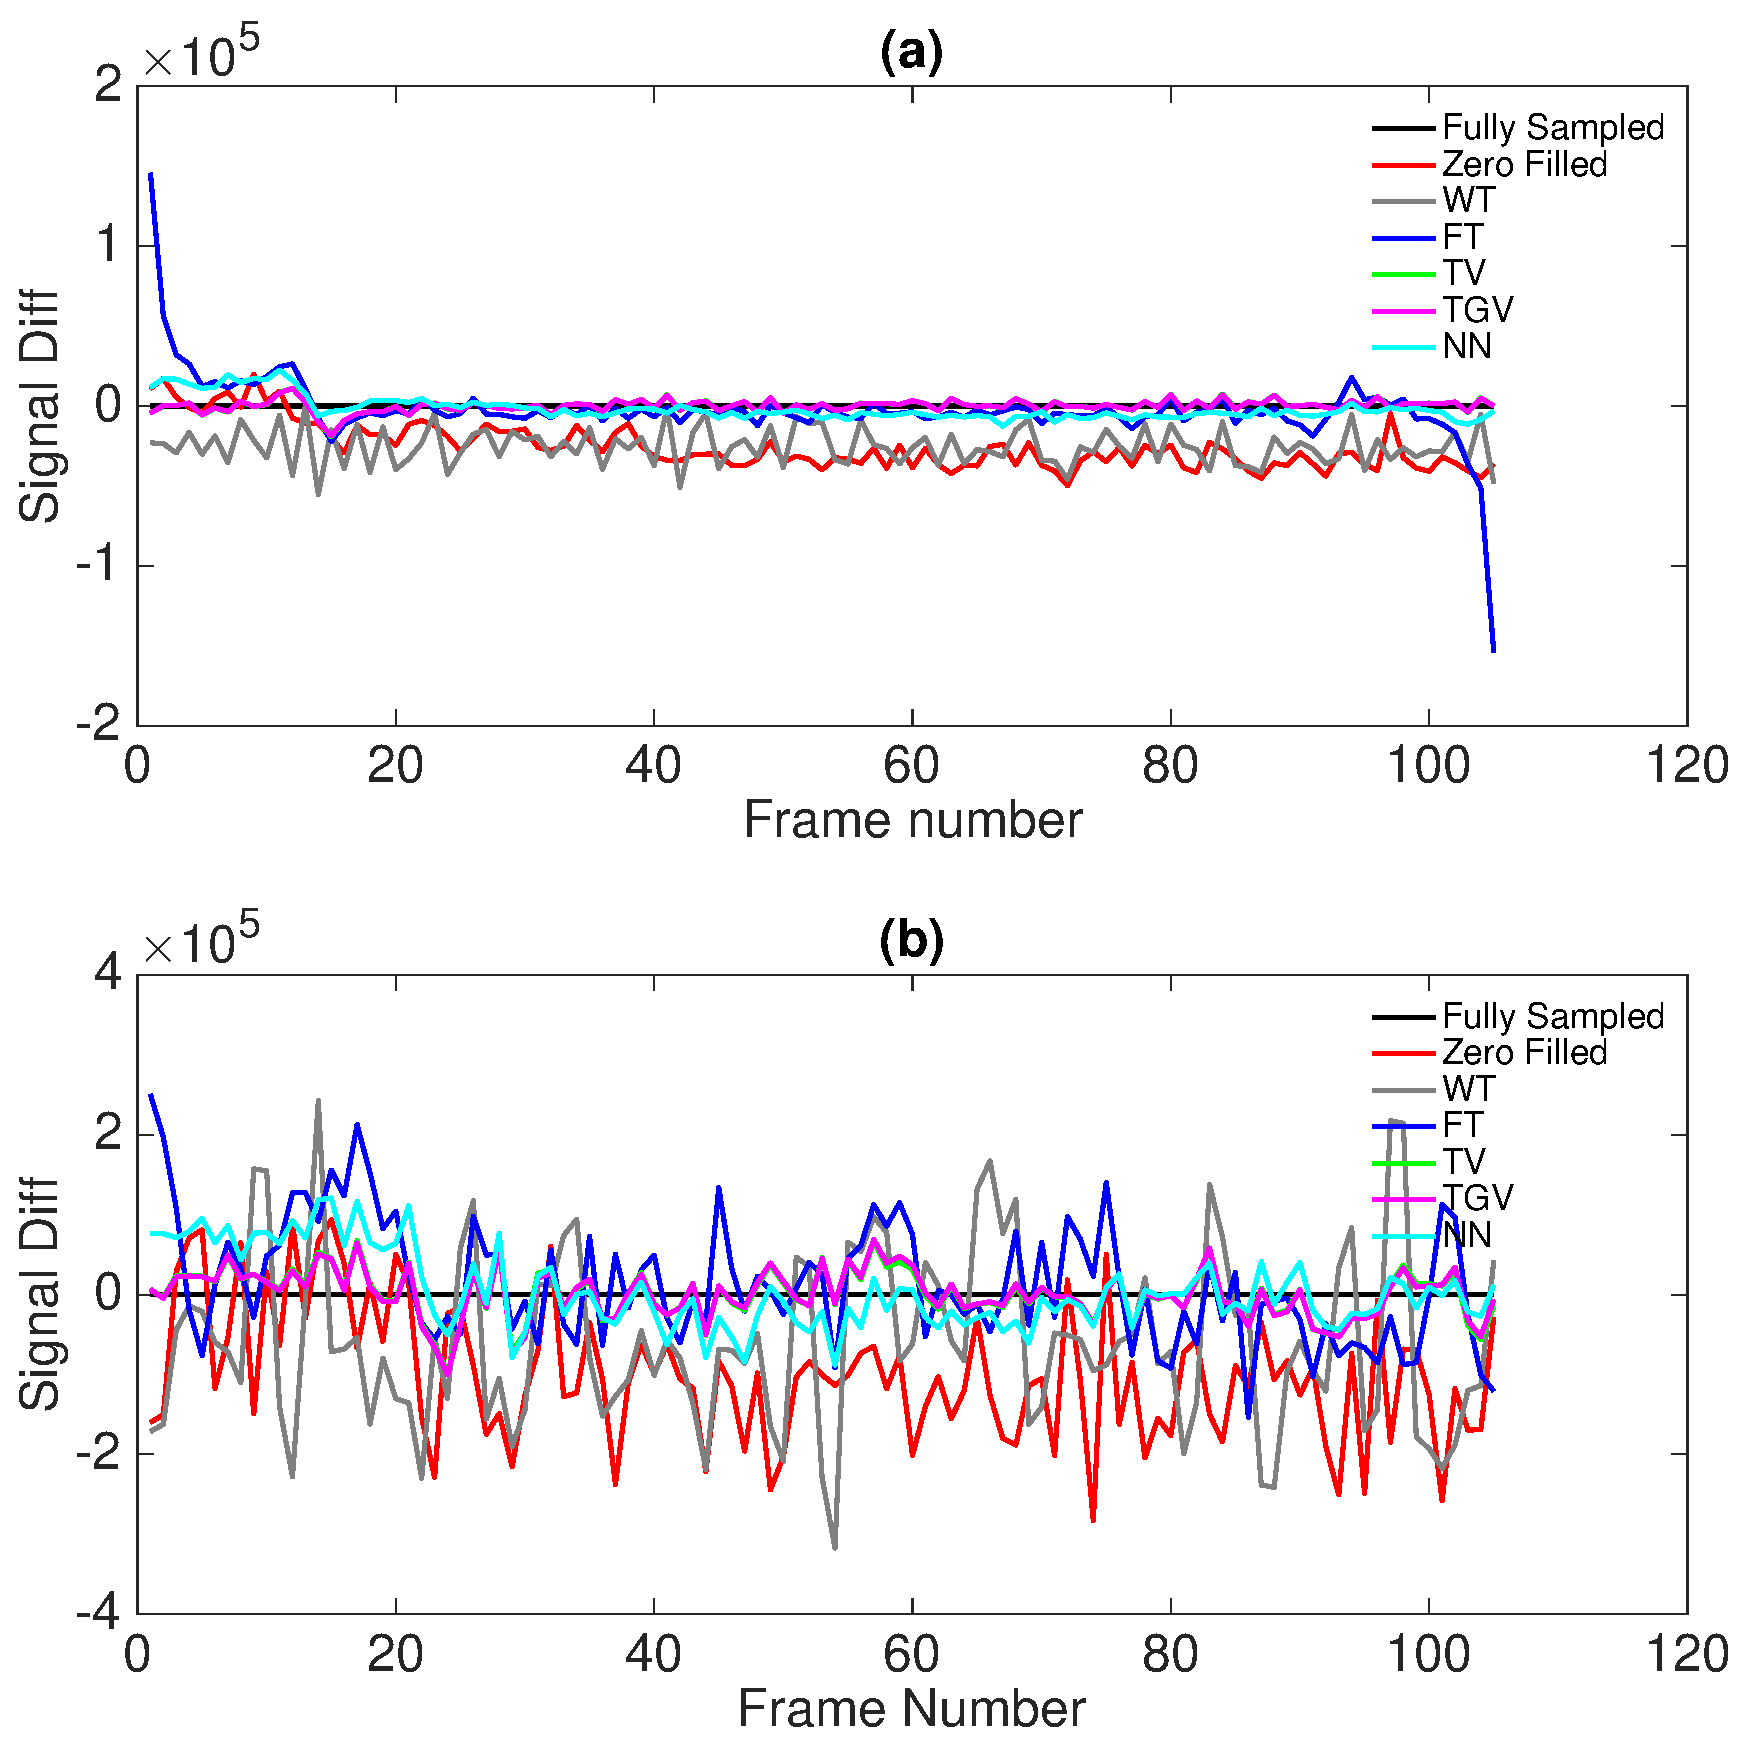
\includegraphics[width=0.9\textwidth]{img/qetsr/figure6.eps}}
\caption{
全采样图像与重建图像肿瘤区域像素时间曲线的比较图。(a)肿瘤区域平均像素值的时间曲线比较;(b)肿瘤中心像素(96,96)的时间曲线比较。图(a)显示Zerofilled图像在注入CA之后低估了肿瘤区域的平均像素值。WT在整体上低估了平均像素值。FT在最初和最后的5帧的时间曲线拟合很差,而且整体上表现出了振荡的效应。TV和TGV$_{\alpha}^2$最好地拟合了时间曲线。NN在注入CA之前高估了平均像素值,并且在注入CA之后略微低估了平均像素值。图(b)表明Zerofilled图像在CA注入之后低估了肿瘤中心的像素值。FT和WT均表现出振荡的效应,使得曲线的拟合变得不准确。TV和TGV$_{\alpha}^2$的时间曲线表现平稳,而NN在注入CA之前高估了肿瘤中心像素值。
}
\label{fig:curves}
\end{figure}

由于在胸部DCE-MRI中,医生更关心参数定量分析的准确性,和SER一样,我们也展示了\kt 和\Ve 的箱型图,如图\ref{fig:paramsbp}所示。在所有的箱式图中,四分位的范围都很小,说明对于胸部DCE-MRI,基于Cartesian采样模式的压缩感知重建有可预测的精度。图\ref{fig:paramsbp}的前两个箱式图可以看出,除了TV和TGV$_{\alpha}^2$,所有结果在统计上都有显著差异。与图\ref{fig:curves}中的发现一致,TV和TGV$_{\alpha}^2$得到了最准确的\kt 和\Ve,其CCC均值高方差小,并且重建图像也最接近于全采样图像。同样,FT在肿瘤均值与CCC方面最不准确,而且肿瘤均值\kt 和\Ve 也与真实值相距甚远。虽然WT也得到了相对准确的肿瘤均值\kt 和\Ve,但其方差较大,说明其可预测性低。

\begin{figure}[htbp]
\centerline{
    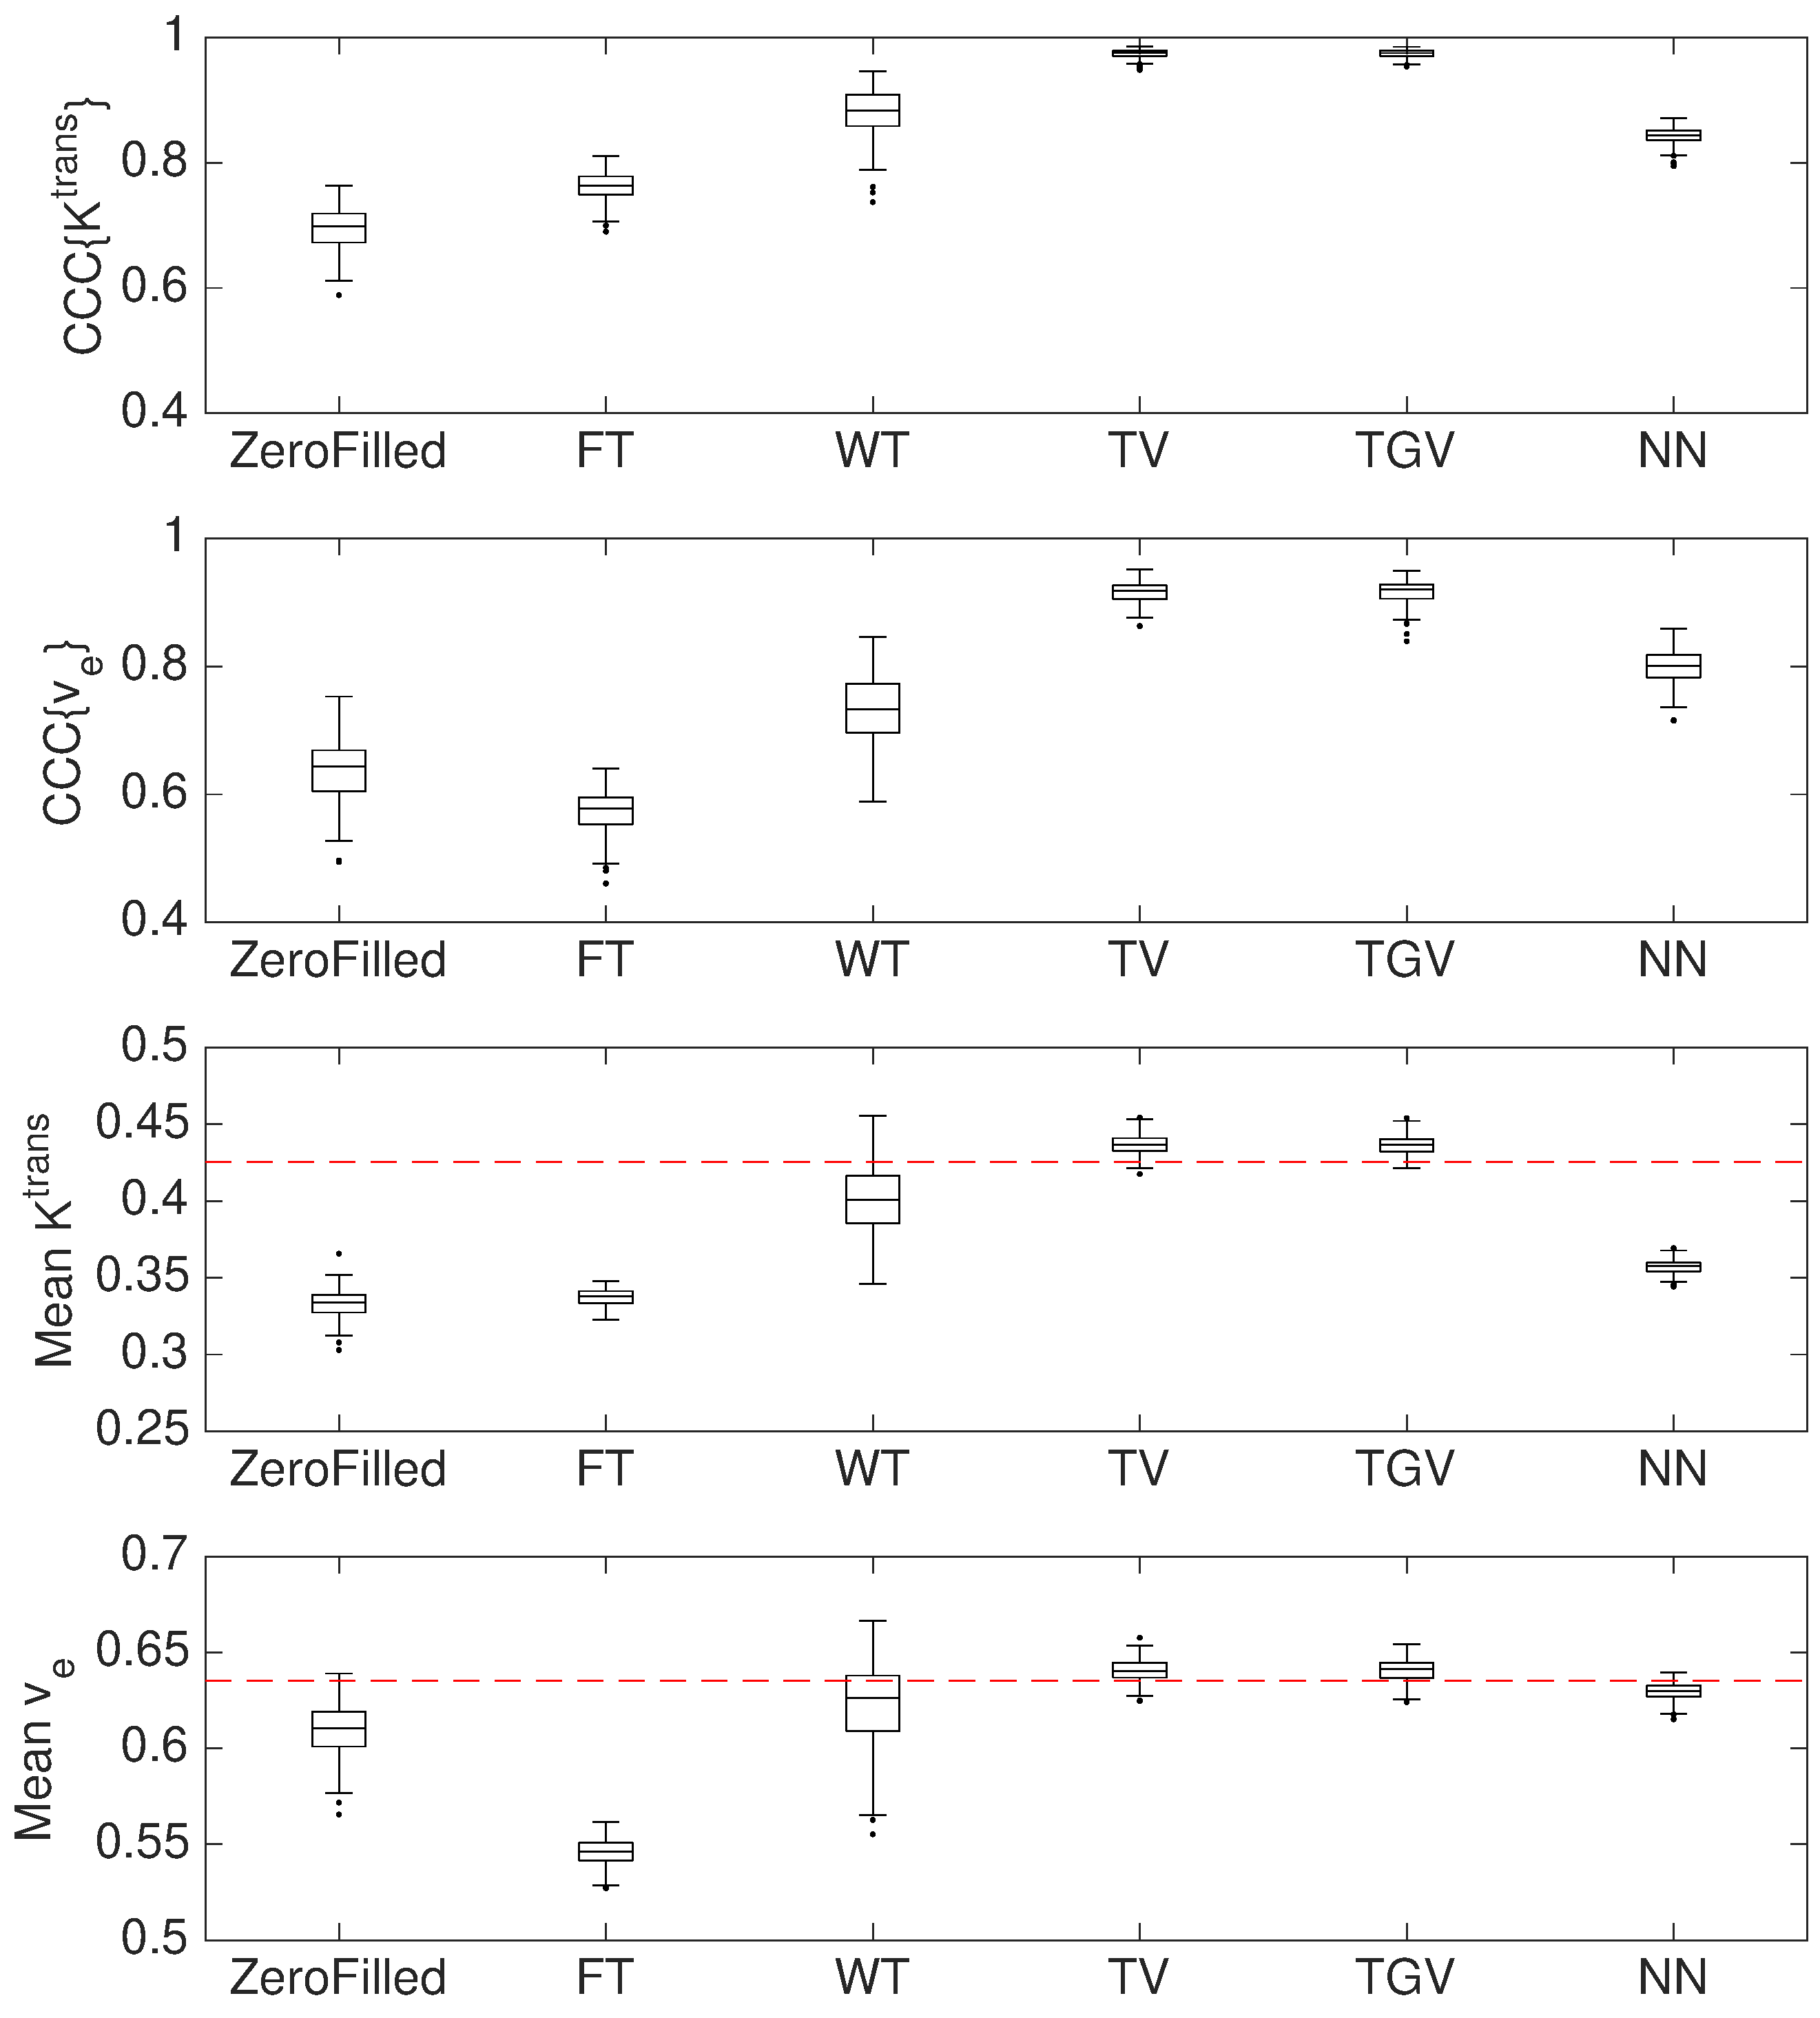
\includegraphics[width=0.8\textwidth]{img/qetsr/figure7.eps}
}
\caption{
200个不同Cartesian采样模式下CCC与肿瘤均值的箱式图。在前两个箱式图中,除了TV和TGV$_{\alpha}^2$,其他稀疏项的重建结果都在统计学上都有显著差异。我们可以观察到,TV和TGV$_{\alpha}^2$得到了最高的CCC,这也和表\ref{tab:params}的结果一致。在后两个箱式图中,红色的水平线代表肿瘤平均\kt 和\Ve 的真实值,分别为0.425和0.635。与表\ref{tab:params}的结果一致,TV和TGV$_{\alpha}^2$得到了最准确的肿瘤平均\kt 和 \Ve,也与真实值最接近。有趣的是,NN倾向于低估\kt 的值但是却相对准确地得到了\Ve。
}
\label{fig:paramsbp}
\end{figure}

\section{数值实验分析}
定量分析表明了5种时间方向的稀疏项在胸部DCE-MRI的压缩感知重建中表现的不同。其中,TV和TGV$_{\alpha}^2$得到了最准确的\kt 和\Ve ,并且它们在肿瘤区域的时间曲线也最贴合真实值。这表明拟合像素值时间曲线的误差可以预测最终量化参数的精度。如果是这样,在没有真实值的前瞻性成像实验中,我们可以用拟合的残差来估计参数的精度。

图\ref{fig:paramsbp}中的箱式图表明,TV和TGV$_{\alpha}^2$之间没有显著性差异,所以很难区分这两种稀疏项在实际中的应用。但由于本文只针对胸部DCE-MRI图像,TV和TGV$_{\alpha}^2$可能在其他部位的图像上有着不同的表现,尤其是当图像存在线性变化的梯度而不是分片常数时。

本文给出的定量参数分析结果应当告知临床并于研究影响重建方法。对于那些需要得到更加精确整体质量的应用,最好的稀疏项选择是NN。而另一方面,如果研究者需要得到更精确的参数分析,最好的选择是TV和TGV$_{\alpha}^2$。

在本文之前,没有工作量化地比较和研究不同时间方向的稀疏项对胸部DCE-MRI压缩感知重建的影响。本文填补了这个空白,但是有三点主要事项。第一,我们在数值实验中仅仅使用了胸部DCE-MRI数据,如果使用其他数据,数值实验的结果和结论可能会有变化,但预计不会很显著。第二,我们在数值实验中只使用了200个Cartesian采样模式,如果使用non-Cartesian采样模式,数值实验结果也可能会不同。第三,FISTA的调参过程是一个不精确的过程,如果使用不同的参数,数值实验结果也可能会有轻微的不同,但我们认为整体的结论是不变的。

\section{本章小结}
在这一章节里,我们针对胸部DCE-MRI图像,量化地比较了5种时间方向的稀疏项在压缩感知重建模型中的表现。我们发现对于胸部DCE-MRI图像,FT是最不适合的稀疏项,因为DCE-MRI图像在时间上没有周期性。WT虽然在参数分析上结果比较精确,但统计上方差较大,而且其重建图像的信噪比最低。NN最好地抑制了由下采样产生的伪影,因此有着最高的信噪比,但是在参数分析上不太精确。TV和TGV$_{\alpha}^2$得到了最精确的参数分析,且二者的结果在统计上没有明显差异。



